\documentclass[12pt,a4paper,fleqn]{article}
\usepackage{rmpackages}																% usual packages
\usepackage{rmtemplate}																% graphic charter
\usepackage{rmexocptce}																% for DS with cptce eval
\usepackage{pdflscape}
%\cfoot{} 													% if no page number is needed
%\renewcommand\arraystretch{1.5}		% stretch table line height

\begin{document}

\begin{landscape}

\section*{Version 1}

\begin{center}
\begin{multicols}{3}

\includegraphics[width=\linewidth]{images/spectrum_black_body_temp3000K_notemp.png}


\includegraphics[width=\linewidth]{images/spectrum_black_body_temp5000K_notemp.png}


\includegraphics[width=\linewidth]{images/spectrum_black_body_temp10000K_notemp.png}
\end{multicols}
\end{center}

\begin{center}
\begin{multicols}{3}

\includegraphics[width=\linewidth]{images/spectrum_black_body_temp3000K_notemp.png}


\includegraphics[width=\linewidth]{images/spectrum_black_body_temp5000K_notemp.png}


\includegraphics[width=\linewidth]{images/spectrum_black_body_temp10000K_notemp.png}
\end{multicols}
\end{center}

\begin{center}
\begin{multicols}{3}

\includegraphics[width=\linewidth]{images/spectrum_black_body_temp3000K_notemp.png}


\includegraphics[width=\linewidth]{images/spectrum_black_body_temp5000K_notemp.png}


\includegraphics[width=\linewidth]{images/spectrum_black_body_temp10000K_notemp.png}
\end{multicols}
\end{center}

\begin{center}
\begin{multicols}{3}

\includegraphics[width=\linewidth]{images/spectrum_black_body_temp3000K_notemp.png}


\includegraphics[width=\linewidth]{images/spectrum_black_body_temp5000K_notemp.png}


\includegraphics[width=\linewidth]{images/spectrum_black_body_temp10000K_notemp.png}
\end{multicols}
\end{center}

\begin{center}
\begin{multicols}{3}

\includegraphics[width=\linewidth]{images/spectrum_black_body_temp3000K_notemp.png}


\includegraphics[width=\linewidth]{images/spectrum_black_body_temp5000K_notemp.png}


\includegraphics[width=\linewidth]{images/spectrum_black_body_temp10000K_notemp.png}
\end{multicols}
\end{center}

\begin{center}
\begin{multicols}{3}

\includegraphics[width=\linewidth]{images/spectrum_black_body_temp3000K_notemp.png}


\includegraphics[width=\linewidth]{images/spectrum_black_body_temp5000K_notemp.png}


\includegraphics[width=\linewidth]{images/spectrum_black_body_temp10000K_notemp.png}
\end{multicols}
\end{center}

\newpage

\begin{center}
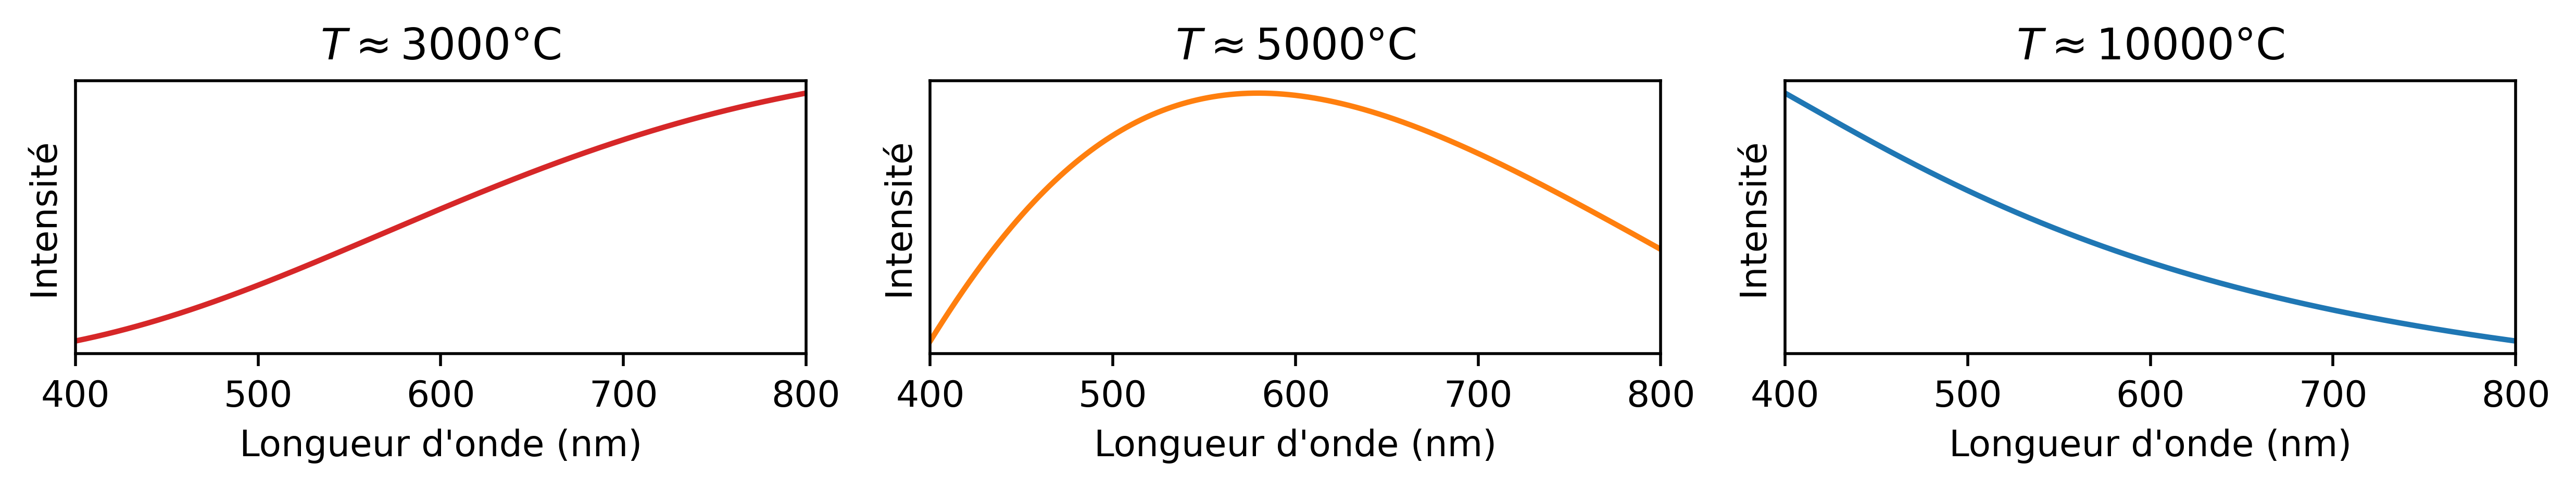
\includegraphics[width=\linewidth]{images/spectrum_black_body_curve10000K.png}
\end{center}

\begin{center}
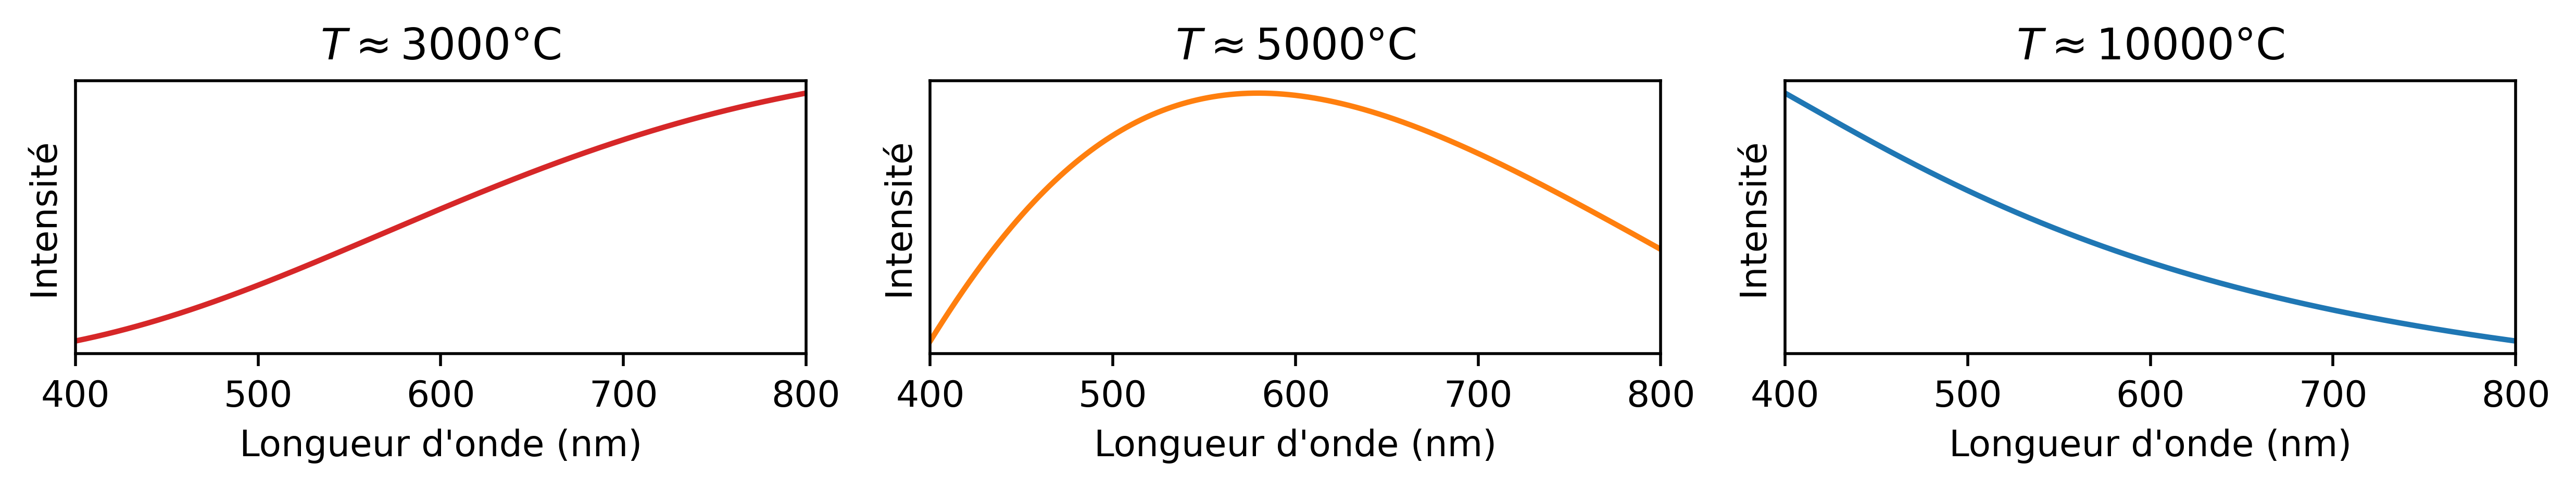
\includegraphics[width=\linewidth]{images/spectrum_black_body_curve10000K.png}
\end{center}

\begin{center}
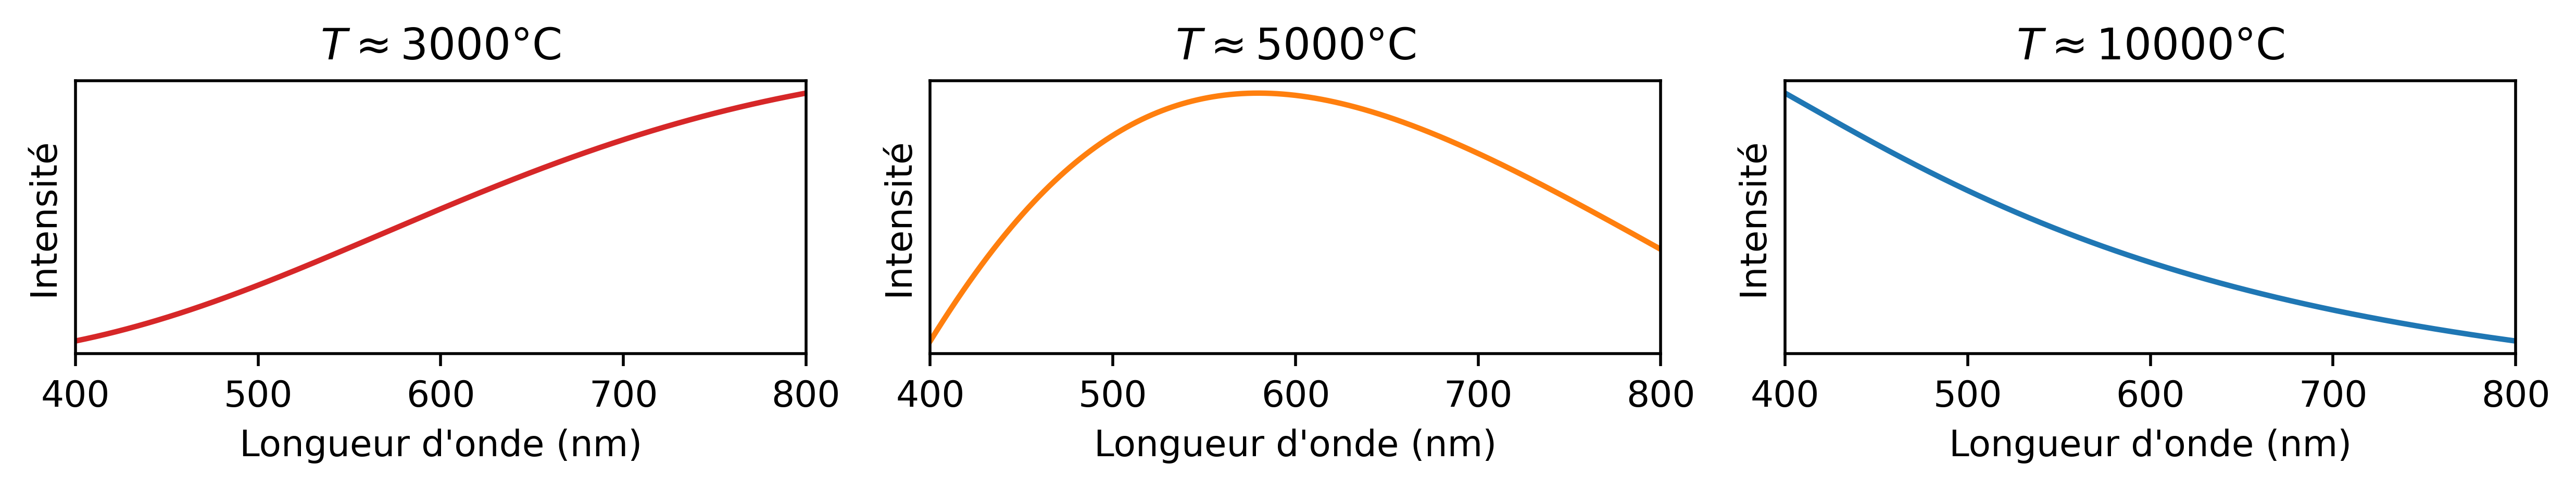
\includegraphics[width=\linewidth]{images/spectrum_black_body_curve10000K.png}
\end{center}

\begin{center}
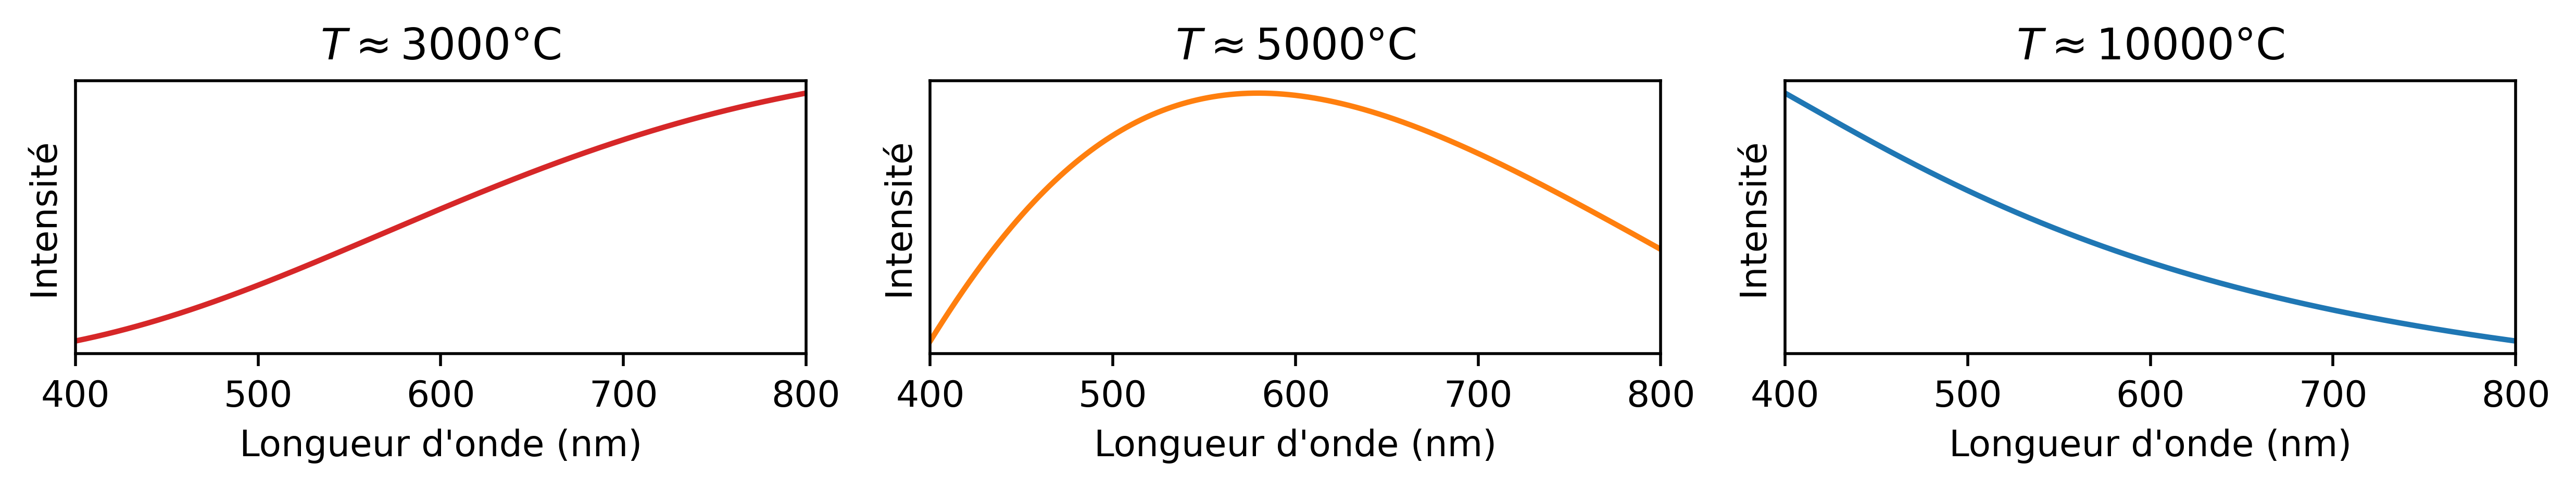
\includegraphics[width=\linewidth]{images/spectrum_black_body_curve10000K.png}
\end{center}

\begin{center}
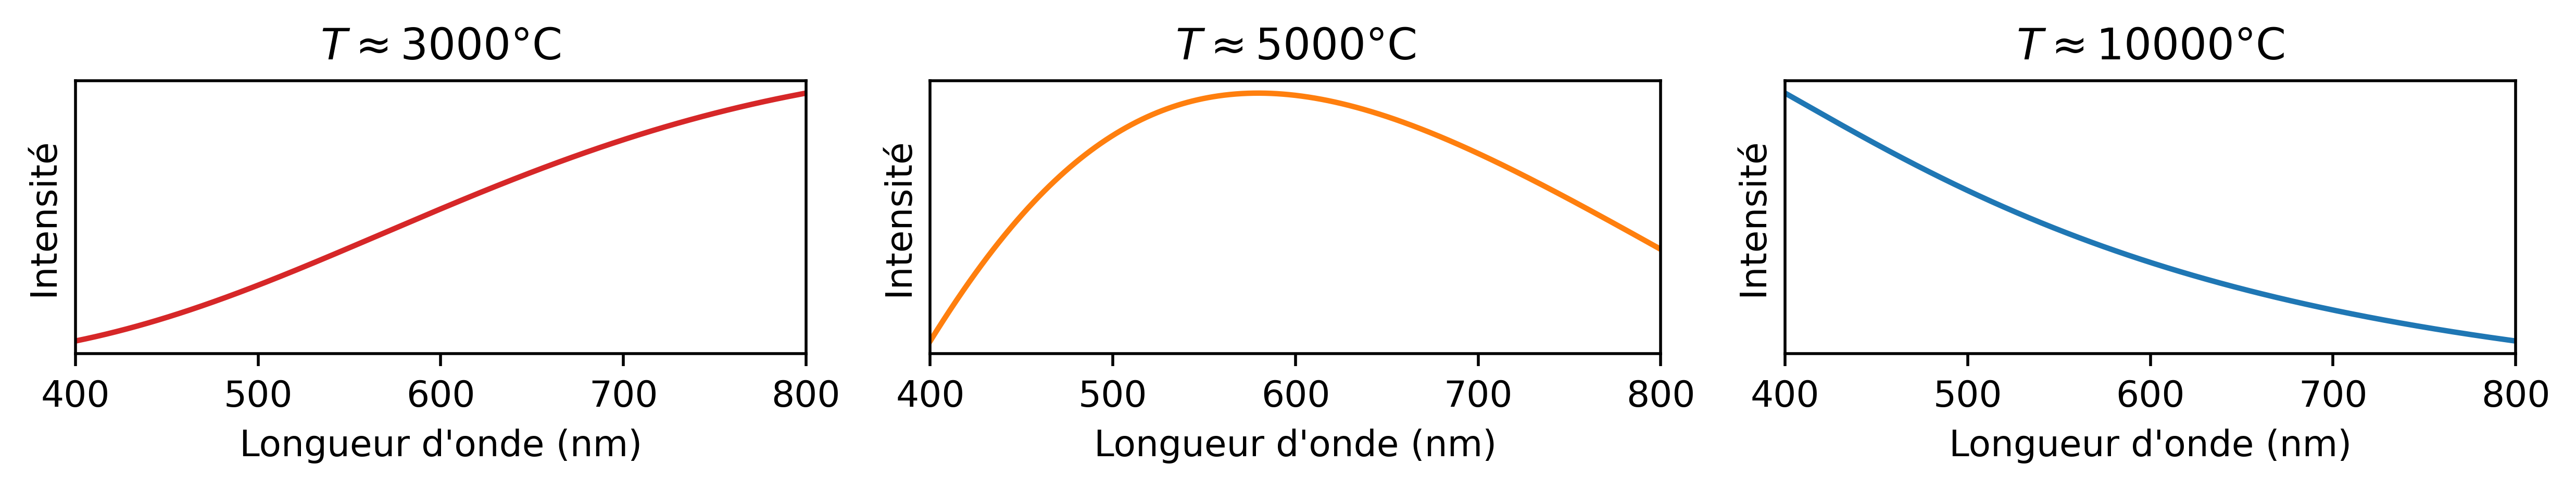
\includegraphics[width=\linewidth]{images/spectrum_black_body_curve10000K.png}
\end{center}

\begin{center}
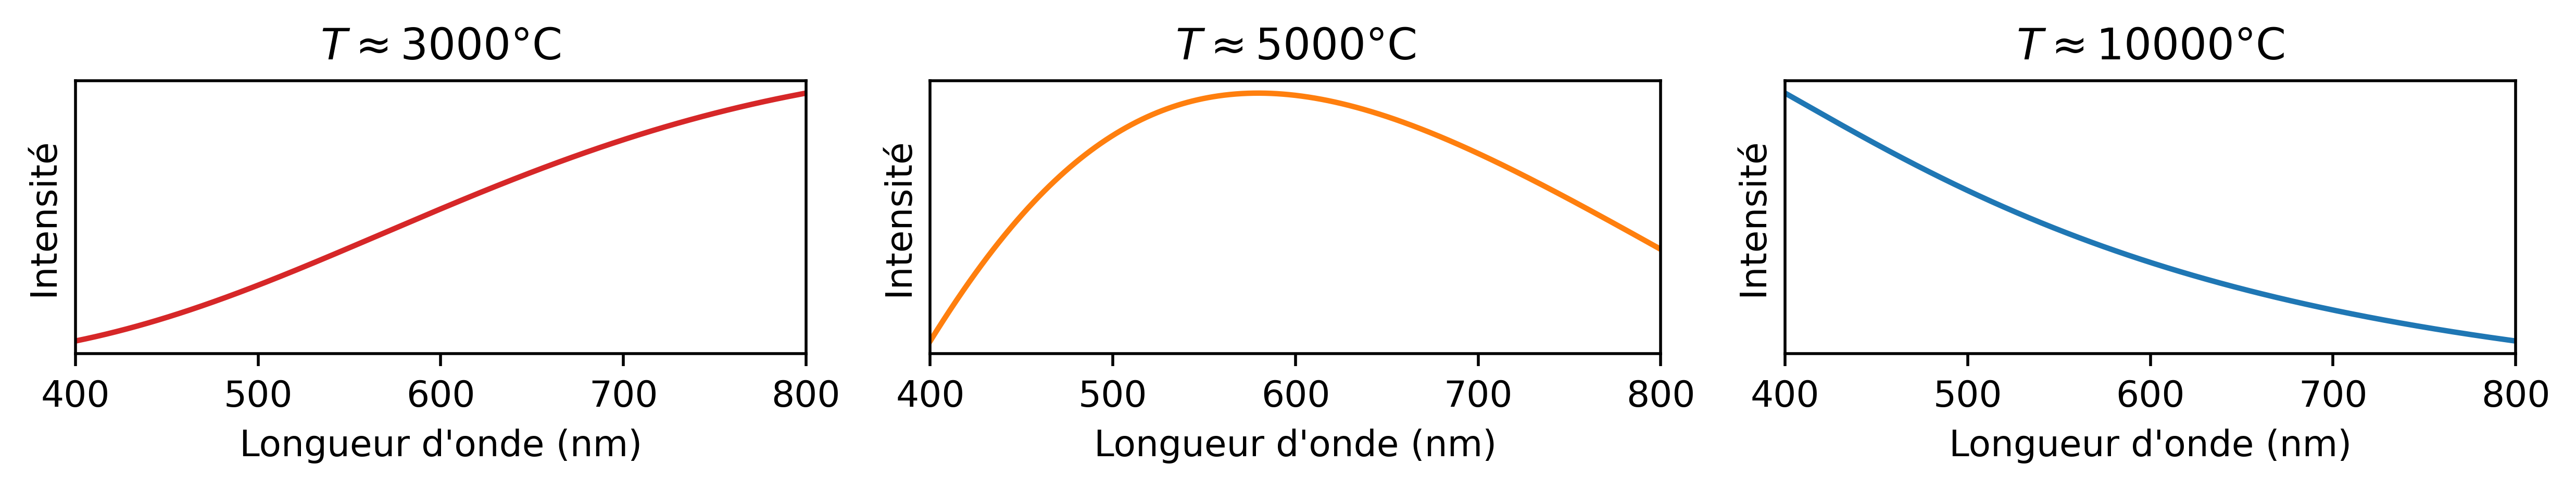
\includegraphics[width=\linewidth]{images/spectrum_black_body_curve10000K.png}
\end{center}

\newpage
\section*{Version 2}

\begin{center}
\begin{multicols}{3}

\includegraphics[width=\linewidth]{images/spectrum_black_body_temp3000K.png}


\includegraphics[width=\linewidth]{images/spectrum_black_body_temp5000K.png}


\includegraphics[width=\linewidth]{images/spectrum_black_body_temp10000K.png}
\end{multicols}
\end{center}

\begin{center}
\begin{multicols}{3}

\includegraphics[width=\linewidth]{images/spectrum_black_body_temp3000K.png}


\includegraphics[width=\linewidth]{images/spectrum_black_body_temp5000K.png}


\includegraphics[width=\linewidth]{images/spectrum_black_body_temp10000K.png}
\end{multicols}
\end{center}

\begin{center}
\begin{multicols}{3}

\includegraphics[width=\linewidth]{images/spectrum_black_body_temp3000K.png}


\includegraphics[width=\linewidth]{images/spectrum_black_body_temp5000K.png}


\includegraphics[width=\linewidth]{images/spectrum_black_body_temp10000K.png}
\end{multicols}
\end{center}

\begin{center}
\begin{multicols}{3}

\includegraphics[width=\linewidth]{images/spectrum_black_body_temp3000K.png}


\includegraphics[width=\linewidth]{images/spectrum_black_body_temp5000K.png}


\includegraphics[width=\linewidth]{images/spectrum_black_body_temp10000K.png}
\end{multicols}
\end{center}

\begin{center}
\begin{multicols}{3}

\includegraphics[width=\linewidth]{images/spectrum_black_body_temp3000K.png}


\includegraphics[width=\linewidth]{images/spectrum_black_body_temp5000K.png}


\includegraphics[width=\linewidth]{images/spectrum_black_body_temp10000K.png}
\end{multicols}
\end{center}

\begin{center}
\begin{multicols}{3}

\includegraphics[width=\linewidth]{images/spectrum_black_body_temp3000K.png}


\includegraphics[width=\linewidth]{images/spectrum_black_body_temp5000K.png}


\includegraphics[width=\linewidth]{images/spectrum_black_body_temp10000K.png}
\end{multicols}
\end{center}

\end{landscape}

\section*{Données}

\vfill{}

\begin{multicols}{2}
\begin{center}
\begin{tabular}{l|c}
\textbf{Étoile} & \textbf{Température (\celsius)} \\
\hline
\hline
Proxima du Centaure	& 2\,700 \\
Tau Ceti							& 5\,000 \\
Rigel								& 11\,000 \\
\end{tabular}

\begin{tabular}{l|c}
\textbf{Étoile} & \textbf{Température (\celsius)} \\
\hline
\hline
Proxima du Centaure	& 2\,700 \\
Tau Ceti							& 5\,000 \\
Rigel								& 11\,000 \\
\end{tabular}
\end{center}
\end{multicols}

\vfill{}

\begin{multicols}{2}
\begin{center}
\begin{tabular}{l|c}
\textbf{Étoile} & \textbf{Température (\celsius)} \\
\hline
\hline
Proxima du Centaure	& 2\,700 \\
Tau Ceti							& 5\,000 \\
Rigel								& 11\,000 \\
\end{tabular}

\begin{tabular}{l|c}
\textbf{Étoile} & \textbf{Température (\celsius)} \\
\hline
\hline
Proxima du Centaure	& 2\,700 \\
Tau Ceti							& 5\,000 \\
Rigel								& 11\,000 \\
\end{tabular}
\end{center}
\end{multicols}

\vfill{}

\begin{multicols}{2}
\begin{center}
\begin{tabular}{l|c}
\textbf{Étoile} & \textbf{Température (\celsius)} \\
\hline
\hline
Proxima du Centaure	& 2\,700 \\
Tau Ceti							& 5\,000 \\
Rigel								& 11\,000 \\
\end{tabular}

\begin{tabular}{l|c}
\textbf{Étoile} & \textbf{Température (\celsius)} \\
\hline
\hline
Proxima du Centaure	& 2\,700 \\
Tau Ceti							& 5\,000 \\
Rigel								& 11\,000 \\
\end{tabular}
\end{center}
\end{multicols}

\vfill{}

\begin{multicols}{2}
\begin{center}
\begin{tabular}{l|c}
\textbf{Étoile} & \textbf{Température (\celsius)} \\
\hline
\hline
Proxima du Centaure	& 2\,700 \\
Tau Ceti							& 5\,000 \\
Rigel								& 11\,000 \\
\end{tabular}

\begin{tabular}{l|c}
\textbf{Étoile} & \textbf{Température (\celsius)} \\
\hline
\hline
Proxima du Centaure	& 2\,700 \\
Tau Ceti							& 5\,000 \\
Rigel								& 11\,000 \\
\end{tabular}
\end{center}
\end{multicols}

\vfill{}

\begin{multicols}{2}
\begin{center}
\begin{tabular}{l|c}
\textbf{Étoile} & \textbf{Température (\celsius)} \\
\hline
\hline
Proxima du Centaure	& 2\,700 \\
Tau Ceti							& 5\,000 \\
Rigel								& 11\,000 \\
\end{tabular}

\begin{tabular}{l|c}
\textbf{Étoile} & \textbf{Température (\celsius)} \\
\hline
\hline
Proxima du Centaure	& 2\,700 \\
Tau Ceti							& 5\,000 \\
Rigel								& 11\,000 \\
\end{tabular}
\end{center}
\end{multicols}

\end{document}